%You can delete all the comments after you have finished your document
%this sets up the defaults for the documents, 12pt font and A4 size. The article type sets this up as such as opposed to letter or memo.

%for the finer points LaTeX see https://en.wikibooks.org/wiki/LaTeX or http://tex.stackexchange.com/

\documentclass[12pt,a4paper]{article}
\usepackage{titlesec} %these are how we import packages, one helps set up footers and title layout
\usepackage{fancyhdr}
\usepackage{titlesec}
\newcommand{\sectionbreak}{\clearpage}
\usepackage{apacite}
% !TEX TS-program = pdflatex
% !TEX encoding = UTF-8 Unicode
\usepackage[utf8]{inputenc} % set input encoding (not needed with XeLaTeX)
\usepackage{graphicx} % support the \includegraphics command and options
\graphicspath{{figures/}}
% \usepackage[parfill]{parskip} % Activate to begin paragraphs with an empty line rather than an indent

%%% PACKAGES
\usepackage{booktabs} % for much better looking tables
\usepackage{array} % for better arrays (eg matrices) in maths
\usepackage{paralist} % very flexible & customisable lists (eg. enumerate/itemize, etc.)
\usepackage{verbatim} % adds environment for commenting out blocks of text & for better verbatim
\usepackage{subfig} % make it possible to include more than one captioned figure/table in a single float
\usepackage[toc,page]{appendix}
% These packages are all incorporated in the memoir class to one degree or another...
\usepackage{algorithm}
\usepackage{algpseudocode}
\algdef{SE}[LOOP]{Loop}{EndLoop}[1]{\algorithmicloop\ #1}{\algorithmicend\ \algorithmicloop}%
\usepackage{listings}
\usepackage{color}
\usepackage{amsmath}
\usepackage{pdfpages}

\usepackage[font=small,labelfont=bf]{caption}

%header and footer settings
\pagestyle{fancyplain}
\fancyhf{}
\renewcommand{\headrulewidth}{0.5pt}
\renewcommand{\footrulewidth}{0.5pt}
\setlength{\headheight}{15pt}
\fancyhead[L]{Matthew Lenathen - 40506678}
\fancyhead[R]{ SOC10101 Honours Project}
\fancyfoot[L]{}
\fancyfoot[C]{\thepage}

\lstset{
	escapeinside={/*@}{@*/}, language=C++,
	basicstyle=\fontsize{8.5}{12}\selectfont,
	numbers=left,numbersep=2pt,xleftmargin=2pt,frame=tb,
	columns=fullflexible,showstringspaces=false,tabsize=4,
	keepspaces=true,showtabs=false,showspaces=false,
	backgroundcolor=\color{white}, morekeywords={inline,public,
		class,private,protected,struct},captionpos=t,lineskip=-0.4em,
	aboveskip=10pt, extendedchars=true, breaklines=true,
	prebreak = \raisebox{0ex}[0ex][0ex]{\ensuremath{\hookleftarrow}},
	keywordstyle=\color[rgb]{0,0,1},
	commentstyle=\color[rgb]{0.133,0.545,0.133},
	stringstyle=\color[rgb]{0.627,0.126,0.941}
}
%this starts the document
\begin{document}
	

	

%you can import other documents into your main one, these layout the Title and Declarations on its own page.
%you might need to change these to \ if your on Microsoft Windows.
\newcommand{\HRule}{\rule{\linewidth}{0.5mm}}

\begin{titlepage}
	\begin{center}

	\HRule \\[0.4cm]
    	{\Large \bfseries Real-Time Cloth Simulation using Extended Position Based Dynamics\par}
	\vspace{0.2cm}
	\HRule \\[1.5cm]

	
    	\vspace{3cm}
	\begin{minipage}{0.4\textwidth}
	\begin{center} \large
        \emph{}\\
        	Matthew Lenathen - 40506678
				
   	 \end{center}
    	\end{minipage}
	
	\vspace{2cm}
    	\begin{minipage}{1\textwidth}
    	\begin{center} \large
        
		Submitted in partial fulfilment of \\
		the requirements of Edinburgh Napier University \\
		for the Degree of \\
        	BSc (Hons) Games Development
    	\end{center}
    	\end{minipage}

    	\vfill

    	% Bottom of the page
	\begin{minipage}{1\textwidth}
    	\begin{center} \large
		School of Computing
    	\end{center}
    	\end{minipage}
	
	\vspace{1cm}
    	{\large \today}


	\end{center}
\end{titlepage}
%{\large Submitted in partial fulfilment of the requirements of Edinburgh Napier University for the Degree of }

\section*{Authorship Declaration}
\vspace{0.5cm}
\begin{flushleft}
I, Matthew Lenathen, confirm that this dissertation and the work presented in it are my own achievement.\newline

Where I have consulted the published work of others this is always clearly attributed;\newline

Where I have quoted from the work of others the source is always given. With the exception of such quotations this dissertation is entirely my own work;\newline

I have acknowledged all main sources of help; \newline

If my research follows on from previous work or is part of a larger collaborative research project I have made clear exactly what was done by others and what I have contributed myself;\newline

I have read and understand the penalties associated with Academic Misconduct.\newline

I also confirm that I have obtained informed consent from all people I have involved in the work in this dissertation following the School's ethical guidelines.\newline
\end{flushleft}

\begin{flushleft} \large
\emph{Signed:} \\
\end{flushleft}

\vspace{.5cm}

\begin{flushleft} \large
\emph{Date:} 
\\
\end{flushleft}

\vspace{.5cm}

\begin{flushleft} \large
\emph{Matriculation no: } 40506678  \\
\end{flushleft}
\pagebreak

\section*{General Data Protection Regulation Declaration}
\vspace{0.5cm}
\begin{flushleft}
Under the General Data Protection Regulation (GDPR) (EU) 2016/679, the University cannot disclose your grade to an unauthorised person. However, other students benefit from studying dissertations that have their grades attached. \newline

\vspace{0.5cm}

Please sign your name below one of the options below to state your preference.\newline
\vspace{0.5cm}

The University may make this dissertation, with indicative grade, available to others.\newline
\vspace{3cm}

\includegraphics[height=2\baselineskip]{figures/sig.png}

The University may make this dissertation available to others, but the grade may not be disclosed.\newline
\vspace{3cm}


The University may not make this dissertation available to others.\newline
\end{flushleft}



\pagebreak

%LaTeX let you define the abstract separately so it wont get sucked into the main document.
\begin{abstract}
Abstract here
% fill the abstract in here
\end{abstract}
\pagebreak

\tableofcontents % is generated for you
\newpage

\listoftables
%generated in same way as figures
\newpage

\listoffigures
%you may have captions such as equations, listings etc they should all appear as required
%these are done for you as long as you use \begin{figure}[placement settings] .. bla bla ... \end{figure}
\newpage

\section*{Acknowledgements}
Insert acknowledgements here
\subsection*{}
	I would like to thank my cat, dog and family.
\newpage

\section{Introduction}
\newpage
\section{Literature Review}
\subsection{Introduction to Cloth Simulation}
Cloth is a major aspect of realistic simulations. Present in many different industries such as: film, games development and virtual reality, cloth simulation is a challenge that combines maths, physics and programming. \\

Cloth simulation is a subsection of Physics-based animation. PBA uses physics and code to create a plausible looking display of realistic effects, e.g. fluid simulations, soft-body dynamics etc. Cloth is defined as a flexible plane of some material or fabric that can move in unique ways, such as bending or stretching. This makes it a challenging and unique problem to simulate accurately. \\

The end goal of a cloth simulation can vary depending on the intended use. In computer graphics, physical accuracy is not the highest priority, the end product is mostly focused on how it looks. This is in contrast to cloth simulations for real-world engineering problems, their focus being primarily on physical accuracy, in order to help them predict real-world scenarios. Real time usage of cloth is also very important in the games industry, and will be discussed later. \\

As it is featured in such a wide range of fields, the literature relating to cloth is plentiful. In this section, many papers, books and articles will be discussed and compared in order to give context to the focus of this project, Extended position based dynamics (XPBD).

\subsection{Brief History of Cloth Simulation}
\label{History}
Cloth simulation is a very active field in research, and has been for a handful of decades. The first graphic models used to mimicking cloth was developed in 1986 by Jerry Weil. Before this, cloth objects were created by mapping textures onto rigid surfaces. His method represents cloth as a 2d grid of 3d coordinates, and focused on simulating cloth held at constraint points, like a draped fabric. \cite{weil_synthesis_1986}. This method didn't allow for cloth movement but it piqued the interest of the graphics community regarding cloth simulation. \\

An important development was made in 1987 by Terzopoulos et al. Their method was a general solution for representing elastic deformable objects like rubber or paper. This method is physically-based, meaning the object is active and can respond to external forces such as gravity or wind. Their paper presented various equations on how objects such as cloth or paper should deform when presented with forces, it also describes how they integrated these equations through time, which is a key topic in simulation. This research laid the groundwork for many more physically based models, and more cloth oriented methods. \cite{terzopoulos1987elastically} \\

As time went on, more ways to simulate cloth were developed, such as particle based systems by Breen et al. in 1992. In particle-based systems, the simulating focused on a series of connected particles, and how they react with each other. The way these particles interacted formed the basis for the cloth dynamics. \cite{breen1992physically} In their paper they decided to move away from continuum based methods and switch towards a particle based model. In 1995, Provot developed a similar particle system but used point masses connected with springs to represent a cloth mesh. \cite{provot1995deformation} \\

In 1998, Baraff and Witkin developed a method that used implicit integration combined with the cloth being represented as a mesh of triangles. This new proposed system allowed for bigger time steps to be taken and faster simulation times. This system is still used today as the foundation for new methods. \cite{Baraff1998largesteps} \\

Later, in 2007, Müller et al. developed and published a paper on a state of the art method for dynamic simulations called Position Based Dynamics. This technique, along with a newer extended version, is the main focus of this project and will be discussed in a later chapter. \cite{muller2007position} and \cite{macklin2016xpbd}

\subsection{Underlying Physics}
\label{Physics}
In order to discuss the advancements and methods within the current literature, it is important to delve into the underlying physics that allow cloth simulations to function. This section will go over important principles that are crucial to creating such simulations.
\\

Often, cloth is represented by particles. These particles have position p, and velocity v, and can be arranged in a grid structure to model a piece of cloth. In order to represent the actual geometry of these particles, they can be arranged into triangles that make up a bigger mesh. When these triangles are small enough, that is when the simulated cloth can look realistic.
\\

For simulations such as mass-spring systems, forces are the primary mechanism for making the particles move. In this case, spring forces between two particles are calculated using Hooke's law, and they say that if the spring is stretched or compressed more than the springs rest length, forces are applied to remedy that. Other common forces are gravity and wind and these will be applied to near all simulations regardless of if it is a force-based method or not.
\\

As the main focus of this project is position-based dynamics, constraints must be discussed too. Constraints are pivotal to position-based dynamics because instead of relying on forces, PBD directly adjusts positions to satisfy constraints. Constraints can vary depending on the situation but usually there are some staples such as distance, bending and collision constraints. Each of these will ensure that the particles within the simulation act as realistic as possible. 


\subsection{Offline Cloth Simulation} 
Cloth simulation can generally by split into two categories: Offline and Real Time. Offline simulations are calculated, tweaked and edited before being rendered to the screen. Commonly used in film and animation, visual fidelity is of utmost importance. Offline calculations can also help in a real time scenario by precomputing effects. \\

\subsubsection{Fine Cloth Interactions}
As offline simulations are not limited by the time between each frame, they can afford to focus on realism. They can do this by scaling the number of triangles up and allowing for finer interactions like folding and wrinkling, these interactions being crucial to a convincing cloth simulation. A great example of such work is presented in a paper by Selle et al., they detail their method of creating a high resolution simulation with up to two million triangles, that can accurately capture the intricate details of cloth. \cite{4522545}\\

At the time of publication, cloth simulations were adding physically-based interactions like wrinkles through a separate modelling system. This can be seen in the work by Cutler et al., in which they created a system that allowed the artist to add in wrinkles on top of an existing character's clothing \cite{10.1145/1073368.1073384}. They achieved this by splitting it into stages: wrinkle creation and wrinkle evaluation. In the wrinkle creation phase, the artists use a tool to create winkle patterns, which get turned into a set of forces on the surface. Next, in the wrinkle evaluation phase, the system generates these deformations based on character poses, and the artists can either choose to keep these generated wrinkles, or alter the pattern until satisfactory results are achieved.\\
In their results, they were able to use their system to create clothing wrinkles on hundreds of characters for a feature-length animated film. They noted that in production, close to zero hand-tweaking was needed for the wrinkles, proving its reliability.\\
When discussing their work, they did note that the visual results from a dynamic clothing simulation is much preferred to what they achieved with their kinematic wrinkle system. This is where the work of Selle et al., aims to improve upon. \\

In their paper, they aimed to create a system where fine details such as folds and wrinkles were created in a physically-based fashion, from the various forces acting on the cloth. Their setup included a mass-spring system with edge and bending spring, and a modified time integration scheme. One notable contribution from their work is how they handle collisions. They note that in order to achieve high resolution folds and wrinkles, the self collisions and interactions must be extremely robust, as they are what cause cloth to create these effects in the first place. In their paper, they created a hybrid repulsion/collision technique that works based on the last known collision. They also utilise parallelism to further improve computing times.\\
In their initial evaluation, the researchers put their system to the test with a twisted cloth model comprising 500,000 triangles.  This example took an average of 30 minutes to calculate each frame. They found that their system was able to simulate an extremely detailed cloth with accurate folds and wrinkles, alongside realistic collision and repulsion. These advanced and realistic effects lend themselves to the offline nature of the simulation, as calculating all of these effects are extremely computationally expensive.

\subsubsection{Precomputing Cloth Effects}
In computer graphics, it is often said that precomputing everything is simply not viable due to how many interactions can occur, but in a paper by Kim et al., they discuss precomputing secondary cloth effects. \cite{kim2013near}. In this case, secondary cloth effects refer to things such as folds and wrinkles, these are expensive simulate in real-time. In this paper, they propose a method to use many thousand CPU-hours to calculate these advanced effects in advance, based on a character motion graph. They achieve this by representing a character with two motion graphs, the primary graph simply being the movement of the character, and the secondary being the cloth dynamics. \\

To evaluate their method, they acquired 12 unique motion clips for the primary graph, and used ARCSim cloth simulator for the cloth motion. They found that in their massive precomputation, they were able to generate good looking cloth animations for any random paths through the primary graph. Initially their secondary graph was just one to one mapping of character poses to cloth, but this proved insufficient for realistic motion, so the secondary graph was made much more complex. 
Overall, the inclusion of precomputing cloth motion, helped simulate incredibly detailed secondary features of cloth, such as wrinkles and folds. This research also links into game development in their discussion section, they propose that viewing a database of precomputed cloth motion could be a great benefit when creating games, as certain scenes could be viewed and edited, also bad looking cloth could be fixed by hand to help realism within the game. \\

In summary, it can be seen that offline simulations, compared to real-time, prioritise visual plausibility and realistic effects. These simulations can be achieved due to their non-real-time nature, being able to compute all necessary effects in advance, and being able to tweak things that don't quite match with others. Making offline simulations great for things such as: animation, fashion design and the film industry. This level of details contrasts with real-time simulations, where they must balance out visual quality with the demands of immediate computation.


\subsection{Real Time Cloth Simulation}
Real time cloth simulations are created by computing the cloth dynamics at runtime, allowing interaction with the user through input and changes from the environment. As the time between frames on real time applications is small, the dynamics need to be calculated and applied efficiently, usually on the GPU. The most common use case for real time cloth simulations are in video games, and as these games also have lots of other calculations going on in the background, means optimisation is even more important. This section will discuss the literature on methods to create these simulations and how they compare with each other. \\
\subsubsection{Mass-Spring Systems}
\label{Mass-Spring}
As mentioned in section \ref{Physics}, mass-spring systems are a popular approach to cloth simulations. They represent a cloth as a grid of particles that can exert forces on each other. The way they exert forces are through springs. The first example of this system, as noted in section \ref{History}, was introduced by Provot \cite{provot1995deformation}.\\

In his paper, he posited that the current state of cloth animation at the time had a lack of realism, especially in the realm of elasticity. His proposed mesh had three different types of springs to achieve different effects. Structural springs being the most basic, it connects adjacent particles in a grid formation. Shear springs connect particles diagonally, and bend springs connect particles by skipping a particle in between, e.g. connecting particle [i,j] to particle [i+2,j+2]. \\

This research successfully modelled a more realistic cloth using mass-springs and inspired research into more efficient mass-spring systems for use in real time, such as the work by Kang and Cho \cite{kang2012photorealistic}. It is known that the mass-spring model suffers from instability, especially at larger time steps, Kang and Cho aim to resolve this instability by proposing a more stable and accurate integration model. They note that an implicit integration scheme would help stabilise the system but it cannot be easily parallelised, so an improved explicit method was chosen. \\

It is noted that Hooke's law is commonly used with mass-spring systems to calculate forces, but Kang and Cho decided to use a harmonic oscillation model, allowing for integration.\\
With their new integration method and parallelism implemented, they were able to simulate cloth containing 16,384 particles and 161,544 springs at  over 68 frames per second. This shows that mass spring systems can be a good tool for simple simulations, although in their results they also show that once the springs get to a large size, in this case 1,200,000 springs, the frame rate drops to 15. It can be seen in current day simulations that the additional complexity from all the springs, stiffness tuning and overall accuracy lead to mass-spring systems not being the optimal method for real time cloth simulations.

\subsubsection{The Continuum Model}
While representing cloth with particles and springs can be straightforward and relatively pleasing to look at, there is a downside to this method, the real world representation of cloth. It is very hard to come up with a spring model that accurately represents various cloth materials such as nylon. This is where the continuum system for cloth fits in. The continuum method treats cloth as a continuous material made up of triangles rather than particles with space in-between, and instead of looking at spring forces, continuum looks at how each triangle is stretched and compressed. \\

As mentioned in section \ref{History}, Baraff and Witkin proposed one of the first continuum models in their paper \cite{Baraff1998largesteps}. A few others attempted such models such as \cite{terzopoulos1987elastically}. Although in their implementation, the damping forces weren't explored in much depth. Another paper by \cite{carignanclothy} built upon the work by Terzopoulos et al. and improved the damping forces by adding a force that damps cloth stretch and shear. They used an explicit integration scheme so was unfortunately limited by small time steps. These works lead Baraff and Witkin to develop their model. Their goal was to come up with a method that allows for larger time steps to be taken in simulation, as most at the time were bottlenecked by small time steps to remain stable. In their method, they employ an implicit integration scheme which allowed for much better performance, when combined with the simple formulation of internal forces. With this continuum representation, they were able to successfully model the common forces like shearing, bending and stretching. \\ 

In their results, they tested multiple setups including clothing. They found that changing the bend stiffness factor, didn't affect in running times a great deal, which explicit simulators wouldn't be able to do. They were also able to estimate their performance in terms of number of particles, and found that it was slightly better than \(O(n^{1.5})\) which was what they expected.\\

This paper laid the groundworks for many continuum implementations, one of which being a paper on data-driven elastic models for cloth simulation \cite{wangdatadriven}. Their goal was to more closely represent how different materials are simulated, ideally close to their real world counterpart. It does this by representing cloth with a piecewise linear elastic model. They explain that real world cloth items such as clothes often have anisotropic properties from the woven nature of cloth, and that this is often ignored by most cloth simulations for simplicity. A part of their research was a way to measure real life samples of cloth, construct a database of parameters are use them directly in their cloth simulation which was a very interesting way to get realistic results.
\\

Finite element analysis is a way to break down the cloth into discrete elements such as triangles, and the physical behaviour is calculated based on the material properties and forces acting on it. In 2020, Kim discussed how most cloth simulation are either made from finite element methods, position based dynamics or mass-spring systems, and that the Baraff-Witkin model doesn't really fit into these categories. In his paper he formulated a version of the Baraff-Witkin model but entirely in terms of finite elements \cite{FEMcantunderstand}. \\ 


\subsubsection{Cloth Simulation with Camera Capture}
As cloth simulation is such a wide field of research, there are many alternative methods and interesting papers to look at, one such idea is SimulCap by \cite{Yu_2019_CVPR}. SimulCap is a method of capturing human movement while also capturing dynamic details such as folds and wrinkles. It uses a RGBD (RGB depth) camera. Their problem with other recent implementations were the lack of realism, in part due to the human and cloth being considered as one piece of geometry, and also the results not being editable, which is a huge aspect of a lot of use cases, i.e. virtual dressing applications. So, for SimulCap, the authors decided to combine a layered representation of the human body, while also having a separate cloth simulation that matches the human movement. For their cloth simulation, they chose to use a mass-spring model for simplicity and also an explicit integration scheme with a small time step for stability. In their results, they compared their implementation with DoubleFusion, another previous system by \cite{yu2018doublefusion}, which is a state-of-the-art system for real time human capture. The authors found that SimulCap achieves a much more realistic cloth representation, mainly due to the separation of geometry as described earlier. The limitations of this system lie in the variation of clothing, e.g. thick jumpers remain challenging to simulate, also due to the simple nature of the cloth simulation, the realism could be improved upon by choosing a more advanced technique. \\

In a more recent paper by Wang et al., in 2023, they address the problem of extracting cloth movement combined with clothing motion, by proposing a novel method of capturing the human motion and clothing separately using double layer neural radiance fields (NeRF) \cite{Wang_2023_CVPR}. NeRF is a method of reconstructing a 3D scene using sparse 2D images. This is makes it a perfect method for cloth simulation using camera capture.During the optimisation phase, they introduce a physics-aware cloth simulation network to properly handle the cloth dynamics to ensure realism.

They comment on the previous implementation, SimulCap, by saying it failed to track the motion of the clothing to achieve editable clothing on humans, which is a prerequisite to most VR/AR apps. Their solution, using NeRFs, model both the body and the clothing in template space, which can then be transformed into observation space using deformation fields. Then, using the two NeRFs from before, the rendered images can be synthesized.

This approach addresses the problems with previous camera capture implementations. Its physics network is taught from simulation data, to constrain the clothing and ensure physically plausible clothing deformations.
In their comparison to state of the art methods, which include DeepCap and NerfCap, they found that their implementation vastly outperformed the other methods without a cloth template, and achieved a much higher accuracy during geometry tracking.


\subsubsection{Cloth Simulation with Neural Networks}
\label{neuralSection}
Another interest alternative method to cloth can be found in the research of \cite{neuralCloth}, a cloth simulation framework that uses an unsupervised deep learning methodology. This has been attempted in the past but the other approaches do not handle cloth dynamics. The authors note that while supervised learning systems have been used before, it requires huge volumes of data, and it has to be repeated for every garment/body, so they chose an unsupervised approach. For their cloth representation, they chose to use a particle based system that also considers external forces like wind and collision, this cloth is then skinned to a 3D model. After training their model, they compared their results to other unsupervised approaches such as \cite{bertiche2021pbns}. They evaluated their framework with multiple different body motions such as jumping and spinning. They found that their approach was the only one capable of achieving dynamic cloth effects. In terms of limitations, unsupervised learning compared to supervised takes much longer and is more computationally expensive, and neural cloth has yet to implement cloth self-collision which is a crucial component of most simulators.
\\

Another example of cloth simulations using neural networks can be found in the works of Oh et al., where they propose a hierarchical cloth simulation method that combines traditional physical based methods with deep neural networks (DNN) \cite{OhNeural}. They note that proper physically based cloth animation is expensive, so being able to utilise DNNs to replace the complex computation with data inferred from the network will reduce the cost significantly.

Their proposed method would split the simulation into two parts. Firstly, a low resolution or coarse model of the cloth is calculated using a normal physically based method. Then, the DNN is used to calculate the finer levels of the cloth, reducing the computation cost. They note that due to only calculating the coarsest level of cloth using a physically-based method, the overall cloth simulation won't be as accurate as a fully physically-based model but it successfully prevents errors stemming from the DNN, and guarantees a reliable simulation. This can be seen in Figure \ref{fig:DNN}.
\begin{figure}[h]
	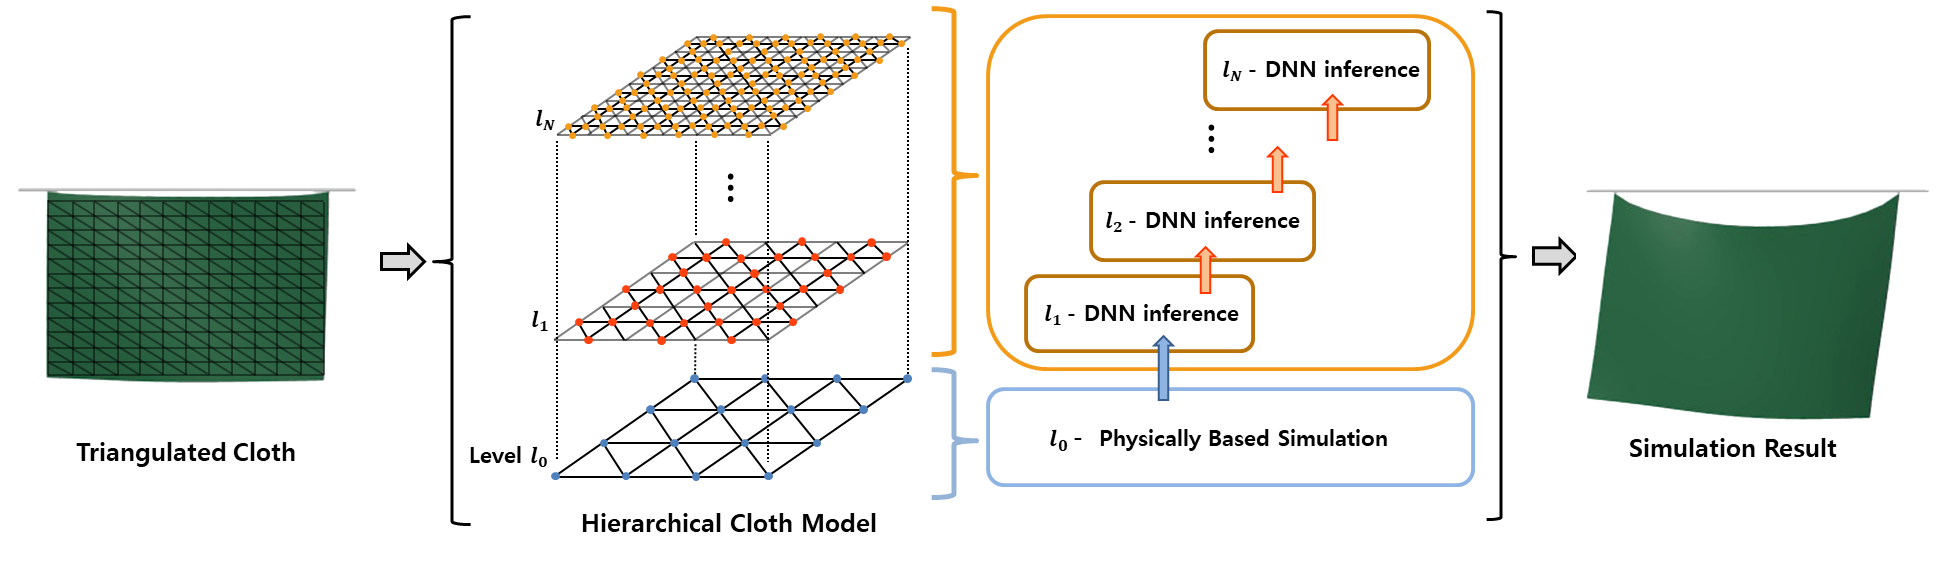
\includegraphics[width=\textwidth]{DNN.png}
	\caption{An overview of a neural network cloth model}
	\label{fig:DNN}
\end{figure}

In their results, they constructed the simulation with three levels, one physically based used projective dynamics, and two DNN models. Projective dynamics will be covered in section \ref{otherMethods}. They compared time performance of their method against a normal implicit integration simulation, and against a projective dynamics implementation with an optimised algorithm applied to it called ADMM (alternating direction method of multipliers) \cite{ADMM}. They found that their hierarchical model that uses DNN improved performance, especially on configurations with many particles, e.g. flags and curtains. They do admit that the accuracy is not on the same level as completely physically based implementations but the results generated were of a high standard and were fast to generate. One final thing to note is that if the cloth is overstretched by external forces, the DNN can sometimes give unusual wrinkles near the bottom of the cloth. They aim to improve this in future work by updating the DNN model to also hold information such as velocity and momentum.


\subsubsection{Shape Matching}
Shape matching is a technique that allows an object to deform but tries to maintain the form of the original shape. In 2005, Müller et al., utilised shape matching to come up with a new method to simulate deformable objects \cite{ogshapematching}. It does this by replacing energies by geometric constraints, and forces by the distance of current positions to goal positions. These goal positions are determined by shape matching, given a rest state. They mention that because the points are always drawn to goal positions, the overshooting issue with explicit methods is completely removed.\\

In their algorithm, their idea is given a set of particles with an initial configuration, every time step the particles are moved towards their goal position, and these goal positions are determined by the original configuration of the shape. In terms of performance, it depends on the number of points used, and they note it is hard to compare it to another model such as mass-spring systems, as the technique depends on the number of clusters chosen, which cannot be reflected in the other models.\\
Overall, this shape matching approach to simulation provides an unconditionally stable simulation that is inexpensive to compute, although the model is not physically accurate.\\

This research inspired a paper on cloth simulation using shape matching in 2013 \cite{BENDER2013945}. As mentioned before, using shape matching for simulations proved unconditionally stable, so a model specifically designed for cloth simulation was created. They note that normal shape matching approaches that use regions, cannot differentiate between shearing, bending and stretching, which are crucial to represent cloth accurately. To combat that, they introduce a novel approach to use a multi-resolution model instead of region based. This can be seen in Figure \ref{fig:shape}, where a is a nested model that shares vertices between levels, and b is a non-nested model that do not share vertices. The results in this paper use a nested configuration. This multi-resolution model will allow for the simulation of fabrics that have different stretching/shearing stiffness. It is also noted that this method is fast due to it scaling linearly with the size of the cloth. \\

\begin{figure}[h]
	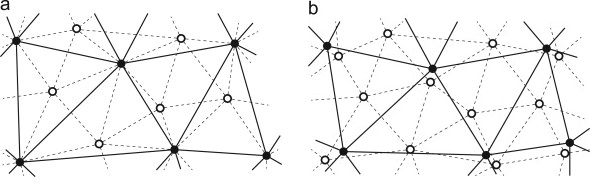
\includegraphics{shapeMatching.jpg}
	\caption{Two levels in a multi-resolution configuration, where a is a nested model and b is a non-nested model.}
	\label{fig:shape}
\end{figure} 
A shape matching approach that used regions was attempted before \cite{regionshapecloth}. But in this model, it introduces forces that influence the bending stiffness and depend on the size of the model, and this is undesirable in cloth simulation. Another problem is that due to small regions within a large model, high stretching and shearing stiffness cannot be obtained. This lead to the development of the multi-resolution approach.\\

In terms of performance, they simulated meshes between 10000 and 100000 triangles to test their scalability, and confirmed their linear relationship between computation time and number of triangles. They also implemented a GPU version of the method which resulted in a much faster compute time. They found in similar setups, the multi-resolution method was around 9 times faster than a standard mass-spring system, and around 15 times faster than a corotational finite element method, a method created by Etzmuss et al. \cite{etzmuss2003fast}. Overall, the multi-resolution approach provided a very noticeable speed-up compared to other approaches, at the cost of physical accuracy.
\\

Another implementation of shape matching was proposed by Vassilev, using shape matching to improve upon a traditional mass-spring model \cite{shapeMatchingMassSpring}. Once shape matching is applied, the springs no longer follow Hooke's law but the stability of the simulation is much improved at larger time steps. At the base, this model is based on the work of Provot, discussed in section \ref{Mass-Spring} \cite{provot1995deformation}. The modification made is replacing Hooke's law with shape matching. Vassilev was inspired by the work of Müller et al, in their original shape matching paper, but instead of shape matching on regions of vertices, Vassilev used it on springs. Each mass connected by one spring will have its own goal position to try to achieve. \\
After implementing it in OpenGL with compute shaders, the implementation was tested on a human figure wearing jeans, to monitor the stability of the shape matching springs. He found that for low time steps, the number of iterations that the shape matching method took to stitch the jeans was roughly the same or slightly higher than the original mass spring model. Since the original model is not stable for time steps above 40ms, the shape matching implementation proved better for larger time steps.

Overall, he found that the shape matching spring implementation was considerably more stable and was less dependant on time steps than the original mass spring system. He proposed this method could be used in real time simulation for things such as trying on clothes on models.

\subsubsection{Position Based Dynamics}
\label{lrPBD}
A great number of techniques discussed above have been force based, and these forces are used to calculate accelerations. Finally these accelerations are integrated to find the velocities and positions of particles. The Position based dynamics (PBD) technique takes a unique approach to physically based animations by omitting the velocity layer and directly working on the positions of particles. \cite{muller2007position} The main advantage is the controllability, the integration instability discussed in section \ref{Mass-Spring} is completely avoided due to the lack of explicit integration. As this is a real time technique, it is greatly suited to games development, as it is very helpful to have direct control over positions of objects within the game.\\

It was noted that even though PBD was the first fully position based approach, there had been other attempts to utilize positions in this way, such as \cite{fisixArticle}. In his approach, Jacobsen manipulated the positions directly using a Verlet integrator. The authors mention that Jacobsen didn't go into depth in terms of constraints, which is crucial in cloth simulation. PBD aims to improve upon it by giving a general approach to constraints.\\

To fully discuss the technique, the algorithm must be analysed. In the algorithm, an object is represented by N vertices and M constraints. The vertices are the particles which have mass m, position x and veloctiy v. The constraints contain a few more properties: cardinality, a function, set of indices, stiffness and a type of either equality or inequality. It is noted that the equality property is satisfied if the function of that constraint is equal to 0, and likewise if it has type inequality, it is satisfied if the function is more than equal to zero. The stiffness affects the strength of the constraints and it ranges from 0 to 1.

\begin{algorithm}
\caption{Position Based Dynamics Algorithm}
\begin{algorithmic}[1]
\ForAll{vertices $i$}
	\State initialize $x_i = x_i^0$, $v_i = v_i^0$, $w_i = 1/m_i$
\EndFor
\Loop
	\ForAll{vertices $i$}\State $v_i \leftarrow v_i + \Delta t w_i f_{ext}(x_i)$
	\EndFor
	\State dampVelocities$(v_1, \dots, v_N)$
	\ForAll{vertices $i$}
		\State $p_i \leftarrow x_i + \Delta t v_i$
	\EndFor
	\ForAll{vertices $i$}
		\State generateCollisionConstraints$(x_i \rightarrow p_i)$
	\EndFor
	\Loop{solverIterations \textbf{times}}
	\State projectConstraints$(C_1, \ldots, C_{M+M_{coll}}, p_1, \ldots, p_N)$
	\EndLoop
	\ForAll{vertices $i$}
		\State $v_i \leftarrow (p_i - x_i) / \Delta t$
		\State $x_i \leftarrow p_i$
	\EndFor
	\State velocityUpdate$(v_1, \dots, v_N)$
\EndLoop
\end{algorithmic}
\end{algorithm}
\newpage
Now it can be broken down to see what each part does. Lines 1 to 3 is just initialising each particle with initial position, velocity and inverse mass. Line 6 is where external forces get added to the system, Müller et al. notes that if gravity is the only external force then the line becomes $v_i \leftarrow v_i + \Delta tg$ where g is the gravitational acceleration. Next, on line 10, the new positions are estimated with a explicit Euler integration step, they are then adjusted in the line 15 loop as many times as needed until all constraints are satisfied. Once completed, the line 18 loop then moves the positions to the calculated position and updates the velocity. 
\\
This algorithm can be classed as unconditionally stable as the integration method in lines 19 and 20 do not use future positions/velocities, but instead calculate physically possible configurations and move the vertices to them.\\

In the paper, the authors also discuss their implementation of a cloth simulator for use in games. Their simulator accepts a triangle mesh and creates two constraints, stretching and bending constraints. Much like the springs in mass-spring systems, these constraints force the positions of the particles to satisfy them in order to continue the simulation, this relates to the loop in line 15 of the algorithm.
\\
To test their cloth simulation, they integrated the method into a game environment and conducted various experiments. They note that a positive to this method is that their bending and stretching terms are independent which can lead to more results when testing values. \\ 
In one of their tests they used one way coupling to link cloth to a stationary object, and two way coupled the bottom of the cloth to a rigid body, it resulted in realistic twisting and swaying, but more importantly ran at more than 380fps which showcases the efficiency of this method. \\
They were also able to test tearing of the cloth. Their tearing process is as follows: when an edge stretches past a threshold value then it is split, with the triangles above being assigned to the original vertex and the lower triangles assigned to the duplicate. They claim this is also extremely stable.\\

Overall, this paper was a very interesting approach to cloth simulation at the time, and influenced a great deal of work into real time cloth, eventually being used in Nvidia's physX software which in turn is used very frequently in game development.

\paragraph{Extended Position Based Dynamics} \mbox{} \\
In 2016, Müller collaborated with Miles Macklin and Nuttapong Chentanez to extend position based dynamics and improve upon the original method \cite{macklin2016xpbd}. Their problems with the original stemmed with iteration count and time step affecting the stiffness of the simulated object, specifically: constraints become stiff as iteration count increases/time step decreases. This effect is discussed in the 2014 survey on position-based methods \cite{bender2014survey}. \\
Their solution to this problem involved creating a new constraint formulation that corresponds to elastic potential energy. It also introduces a total Lagrange multiplier, which is a technique used to find the local maxima and minima of a function that is subject to constraints, e.g. in cloth this could be a distance constraint. This Lagrange multiplier allows the constraints to be solved irrespective of time step.\\

To test this on cloth, they set up the same cloth configuration for PBD and XPBD and compared them. They found that PBD became progressively stiffer as the iteration count increased but XPBD remained consistent. They also found a small downside of XPBD in terms of performance per-iteration, but this was less than 2\% of total simulation time. \\

In the limitations, the authors note that the method is only an approximation of an implicit Euler integrator, but this still creates very realistic real time results. Even so, if the application requires great accuracy, it would be advisable to choose a more traditional simulation method.

\label{otherMethods}
\paragraph{Other PBD methods} \mbox{} \\
\label{t}
In 2012, Kim et al., tackled a problem that all cloth has to deal with: inextensibility \cite{longrange}. At the time, existing methods had to solve non-linear systems which are computationally expensive. The authors proposed a new method, long range attachments (LRA). It is designed with the fact that in computer games, cloth is typically attached to the kinematic body of whatever is wearing the cloth. It uses this to create a constraint and enforce global inextensibility. This method can be applied to existing physics methods such as position based dynamics.\\

This works by creating a constraint on a fixed point, e.g. the part of cape attached to a characters shoulders. It then computes the distance from this particle to other attached particles. If a particle goes beyond a certain radius it is projected back towards the surface of a sphere with the centre of that sphere being the attachment point.
\\

The time taken to handle these LRA constraints scales linearly with the number of attachment points. This can be used to optimise the simulation by pruning certain attachment points. For example, in their cape test, they only choose the closest attachment point to each particle and it shows good results. It gets difficult when working on other shapes and for each configuration, it is recommended to find certain groups of pinned points, e.g. a waistline for a skirt.
\\

In their results, they found that the implementation provided a efficient and simple way to solve the stretching problem of cloth in games. They note that this method is only applicable to cloth applied to characters such as dresses, skirts and capes and that any environmental cloth such as a tissue or paper would see no benefit.
\\

Another interesting approach to position based dynamics is found in the works of Bouaziz et al. \cite{projectivedynamics}. They worked on bridging the gap between position based dynamics, a fast physically inaccurate method, and finite element methods. This lead to robust and efficient implementation that was accurate and supported many different types of constraints. Since continuum methods have the unfortunate side effect of being considerable more expensive than other methods, it would be beneficial to have the accuracy of finite element methods with the efficiency of position based dynamics, this is what projective dynamics aims for. The way they achieve this is by instead of using typical constraints found in position based dynamics, they use constraints derived from continuous deformation energies. With this method they can also perform a local and global optimisation step, meaning that for each element, they project it onto the constraint goal, and at the end the global step combines all of these and finds a compromise. 

This is similar to shape matching, which the authors note. \cite{ogshapematching}. Except in shape matching, the constraint projections are used to create the elastic forces instead of potentials.

When comparing this implementation to PBD, the authors note that the stiffness due to time step problem in the original PBD is solved due to including a momentum term. So that the cloth can behave in a similar way no matter the chosen time step.

When analysing the results, they test a cloth setup as a flag on a pole, which can be seen in Figure \ref{fig:pd}. They used edge constraints and external wind force to simulate movement. They were able to simulate the flag tearing in high wind by removing edge constraints when the strain on the cloth exceeds a certain limit.
\\

\begin{figure}
	\centering
	\includegraphics[scale=0.5]{PDFlag.png}
	\caption{The simulation remaining stable in high wind speeds}
	\label{fig:pd}
\end{figure}

In 2022, Li et al., proposed a new differentiable cloth simulation based on projective dynamics, but with dry frictional contact to simulate cloth self collision \cite{diffCloth}. The key difference of this work is that the simulation is differentiable, meaning gradients can be computed through backpropagation. This means that it can utilise many optimisation methods that result in a great speedup compared to non differentiable simulations. It also aims to  further improve upon the physical accuracy of projective dynamics by adding dry frictional contact. The paper showcases the simulator in many different use cases to showcase the efficacy of it.
\\
One of these examples showcases the usefulness of dry frictional contact, a piece of cloth falling onto a sphere. This is a very standard test in cloth simulation. This example contains both self collision from the cloth and also external contact with the sphere. After colliding the motion was mostly from the frictional component.
\\

Another example is a real-to-sim implementation of a flag. They used real motion of a flag blowing in the wind and tried to create a digital simulation copy. This was particularly challenging as it involved estimating what material was used and also modelling the wind condition at the time. They found it to be a good recreation of it but noted that due to the final loss function being non-zero, it was still imperfect. This is most likely due to the simplistic wind model they employed and could be improved with a more sophisticated model, such as one from a neural network.
\\

When evaluating the implementation, they found that it successfully accommodated rich and detailed self contact, differentiability and dry frictional contact. Since it was differentiable, they were able to utilise backpropagation and observe a significant speedup when compared to other direct solvers. There are a few limitations with this model, one being that since it is based on projective dynamics, it limits the choice of material. Another significant drawback is that the solver doesn't guarantee convergence, even though it is rare for this to happen, it still results in a costly switch to a direct solver. They note that they hope to resolve this in the future.

\subsection{Future Trends}
Since clothing is so prevalent in daily life, the graphics and physics research communities are always striving to improve and innovate the simulation of cloth. The evolution of cloth simulation can and will take many paths. One such path can be seen recently in the works of Clegg et al., which is robot-assisted dressing \cite{robot}. In the future, robots will most likely be interacting physically with humans more, one of these areas could be robot-assisted dressing. As clothing is extremely dynamic, the robot will need accurate cloth simulations to properly assist dressing.
\\

Another possible future trend would be cloth simulations with AI. As previously discussed in section \ref{neuralSection}, there are already examples of cloth simulations using neural networks for constraints. As machine learning and AI techniques improve, we could see more models being trained on real world clothing data and being used in more simulations.
\\

Finally, one more possible future trend is the increasing realism of clothing simulations. As seen in section \ref{t}, projective dynamics utilised the high accuracy of continuum based methods to more accurately simulate clothing. Perhaps in the future, continuum models will improve to accurately simulate a massive range of materials and textures that all have different properties. This would impact most use cases of cloth simulation such as garment try ons, video games and more.
\subsection{Conclusion}
The field of cloth simulation has faced major advancements in the past two decades through a variety of approaches both traditional and novel. Both offline and real-time simulations have seen great improvements through the evolution of methods and by building upon previous works. 
\\

Offline simulation has seen advancements in the form of accuracy and attention to detail. As these simulations are not bound by frame times, they can afford to spend much more time computing effects. This leads to simulations with incredible precision. These are typically seen in animation and film for high visual fidelity.
\\

Real time simulations have also seen big improvements to how they are made. As the use cases for clothing simulations are so large, there have been many different methods to creating simulations, such as camera capture. This is an important step forward as it enables the capture of real life clothing which not only helps to create realistic simulations, but can also be used as data to be fed into other computational models.
\\

Neural networks have also been a big focus for many researchers in the field due to the rapid improvement of AI techniques in recent years. These neural networks can have great predictive capabilities and room to learn off of previous data, which makes it suitable for large or detailed cloth models. Neural network cloth simulations will continue to be improved upon with models holding more data and variables, resulting in more physically accurate simulations.
\\

Despite all of these advancements, the field continues to face hurdles in developing these simulations, such as scalability, computational efficiency and physical accuracy. The future of cloth simulations will likely be solving these problems and discovering new techniques to more accurately model cloth as it appears in the real world.
\\

In conclusion, the literature on cloth simulation reflects a massive field, that is marked by novel and innovate approaches dedicated to improving the realism of cloth simulation. The combination of traditional methods rooted in classical physics, and the interesting techniques in computer science such as neural networks and camera capture highlights the progress of the field to date, but also opens the door to future breakthroughs that will further improve and scale cloth simulations.
\newpage

\section{Methodology}
This section will discuss how various methods of constructing a cloth simulation were achieved inside a physics framework. It will go into depth on the design choices such as which framework to use, programming language and experiment setup. It will also cover the different algorithms used and how they compare with one another. Finally, it will discuss the additional features implemented and how they were useful in evaluating the simulation.

\subsection{Environment and Framework}
Before starting, a choice of which framework to implement the cloth simulation in was required. In this project, a simulation framework is just a sandbox containing the basic necessities for calculating, updating and rendering meshes that are composed of vertices and triangles. In the field of computer graphics/games development, there are a vast number of engines and physics frameworks to choose from. Some of these include: Unity, Unreal Engine, Godot, Nvidia PhysX etc. Research was done into various frameworks but eventually Unity was chosen for this project. \\

Unity is typically used for game development but it is also a very useful tool for building interactive simulations. It has powerful graphics capabilities for shaders and lighting which will highlight the dynamics in cloth well. It also has a massive ecosystem of resources and community support so that any problems or bugs would already be discussed online. Unity also has features that handle collisions, which was useful for implementing a level of interaction where the user can click and drag the cloth around.

\subsubsection{Language Choice}
\label{lang}
Unity's base scripting language is C\#, a high-level object-oriented language. C\# is a managed language, meaning it will only execute while being managed by a common language runtime environment. This provides features such as memory management, garbage collection and security tools. C\# is a common language used in games development but for physics simulations, C++ pulls ahead due to its high performance. C++ compiles straight to machine code which interacts much faster with the hardware it is running on. \\

A base script contains two functions, Start() and Update(). Start is called once at the beginning of the simulation and Update is called every frame. Typically simulations set up all the necessary components such as meshes, colliders and variables in the Start function, and handles the main simulation loop in Update. An important detail about using Unity for physics simulations is the use of a function called FixedUpdate. Compared to the standard Update, FixedUpdate runs at a fixed time interval with a default value of 0.02 seconds, or 50 frames per second. FixedUpdate is necessary for physics simulations due to the amount of complex calculations within them. In this project, Update was only used to handle user interaction with the mouse, and to handle recordings. \\

Typically, Unity scripts will be solely written in C\#, but through the use of dynamic link libraries (DLLs), it is possible to write an external c++ program that is used as a plugin in Unity.

\begin{lstlisting}[caption={Interfacing C++ functions with Unity},label={lst:cppinterface}]
public class cppFunctions
{
	[DllImport("clothsim_dll", EntryPoint = "cpp_init")]
	public static extern void cpp_init([In] Vector3[] vertices,[In] int[] triangles, int numParticles, int numTriangles, float fixedDeltaTime, int algorithmType, int scenario, int solverIterations, [In] int[] staticParticleIndices, int numStaticParticles, int subSteps, Vector3 sphereCenter, float sphereRadius);
	
	[DllImport("clothsim_dll", EntryPoint = "cpp_update")]
	public static extern void cpp_update([Out] Vector3[] vertices,[In] float windStrength, [In] float stretchingStiffness, [In] float shearingStiffness, [In] int selectedParticleIndex, [In] Vector3 mouseWorldPos, [In] int stopGrabbingIndex);
}\end{lstlisting}
Using this class within C\#, allows the user to pass in variables from C\# to C++. This allows for the sections that require excellent performance, the PBD/XPBD simulation loop, to be executed in C++. The simulation loop requires good performance because cloth dynamics require complex calculations on a lot of particles at every frame.\\ 

Variables passed this way can be specified with [In] or [Out] which help specify the direction of data flow. [In] is used for data that doesn't need to be passed back from C++ to C\#, such as the initialisation variables. [Out] is used when data needs to be changed inside C++ and returned to C\#, such as the vertices of the mesh. The vertices need to be passed back to C\#, as Unity needs the new vertices every frame to properly render the cloth while it changes shape.\\ 

The general way this works is that the C++ dll has a cloth simulation object that is created the first time that instance of Unity runs it. It then maintains this object while Unity is open. To get the simulation ready for the next time it is run, all the class variables are reassigned and all the class vectors are cleared. \\

For this project, only the simple mass spring system was implemented in C\#, while all other methods were implemented in the faster C++ code. A boolean flag was used for this, if it was set to C\#, it would execute code in the same script, while if it was set to C++, it would call the cpp\_init function as seen in Listing \ref{lst:cppinterface}. \\

Within the C++ application, the GLM library is also integrated. GLM is a powerful library designed for mathematics in computer graphics \cite{glm}. In this project, GLM is used mainly for its vec3 class, to represent 3D vectors such as position, velocity etc. GLM also contains very useful methods for operating on these 3D vectors such as normalize and length, which are crucial for certain calculations in the pbd and xpbd simulation loops. It is a header only library so the glm folder was simply placed in project directory and added to necessary C++ files with \lstinline[language=C++]!#include <glm.hpp>!.
\subsection{Initialisation}
Initialisation is an important part of the simulation, as it effectively determines the starting state of all objects within it. To start, a cloth mesh is needed. This is typically a flat vertical mesh, meaning it has no depth in the z axis. Initially, a default Unity preset mesh was used for testing. A problem quickly arose where the orientation of the mesh was wrong. This preset mesh was intended to be used as a ground or horizontal surface. When the mesh was rotated horizontally, the y axis became aligned horizontally instead of vertically, which disrupted the physics calculations. Consequently, it was decided to create the mesh from scratch to ensure proper alignment.

\subsubsection{Mesh Creation}
\label{creation}
In Unity, an empty mesh object can be created then filled by the developer to suit their purposes. Meshes require two properties to be set, vertices and triangles. Vertices are just individual points in space, represented by a 3D coordinate. They are used to define the meshes overall structure. Triangles are geometric primitives used to represent the surface of the mesh, and are created by connecting three vertices in a sequence. Another important list is the triangle indices. these indices specify which vertices are used to create a triangle. This is necessary for creating constraints and will be discussed in Section \ref{constraints}. \\

For this project, a mesh generator class was created and holds two functions. GenerateVerticalMesh and GenerateHorizontalMesh. Two parameters are passed to these functions, Grid size and spacing. Grid size represents how many vertices in the x and y axis, e.g. a 20x20 mesh, and spacing refers to the distance between each vertex. For most tests, a 20x20 grid is used with a spacing of 0.5. Creating the vertices is simple, a nested for loop is used and each vertex is set within. The only line within the nested loops is:\\ \lstinline[language=C++]!vertices[i] = new Vector3(x * spacing, y * spacing, 0);!
In the code block, the outer loop iterates over the y-axis coordinates while the inner loop iterates over the x-axis, both from 0 to gridSize. Within the loop this line is executed to generate the coordinate at that index. The x and y coordinates of each vertex are set depending on the current position within the grid, multiplied by spacing to either increase or decrease the space between the vertices. The z coordinate is set to 0 as the cloth has no depth.\\

Generating triangles is a slightly more difficult. For this project, a 20 by 20 mesh will generate 2166 triangle indices, with 722 triangles. The way these triangles are generated is another nested for loop, working on 6 vertices at once and creating two triangles from them. It then moves onto the next 6 vertices. The data stored in the triangles array are the indices of the triangles. \\

Finally, the vertices and triangle arrays are assigned to the mesh object. Additionally, the RecalculateNormals function is called to calculate the normals of this mesh. Normals are necessary for lighting calculations, and they will be recalculated every fixedUpdate. A wireframe of this mesh can be seen in Figure \ref{fig:mesh}.
\begin{figure}
	\centering
	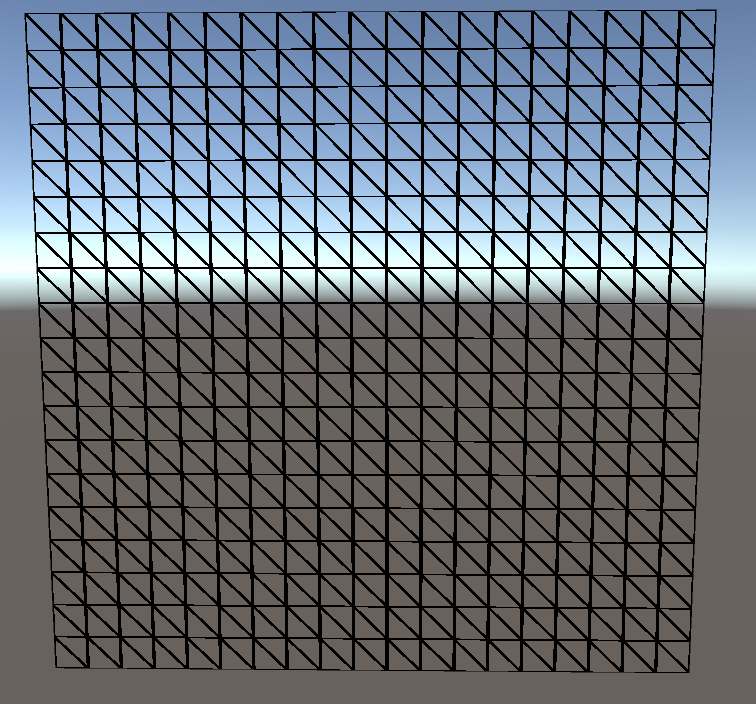
\includegraphics[scale=0.5]{clothmesh.png}
	\caption{A wireframe of a vertical cloth mesh}
	\label{fig:mesh}
\end{figure}
\subsubsection{Particle Class}
One detail that is common to all techniques used in this project is the idea of each vertex being a ``particle". As mentioned in Section \ref{Physics}, vertices can be represented as particles that have various properties. Here, the particle is represented by a class that has 4 properties: $position$, $velocity$, $inverse\ mass$ and $isStatic$. While the first three are fairly self explanatory, the last $isStatic$ property determines whether that particle is fixed in space, and is a boolean. This $isStatic$ variable is very useful for cloth as it allows for certain particles to be pinned, e.g. a hanging curtain or attachment points of a cape to the back of a character model. \\

One important part of initialisation is looping through all the vertices of the mesh and adding them to a particle list. In this loop, particles are assigned the position of the vertex, an initial velocity of 0, an inverse mass of 1.0 and $isStatic$ set to false. Directly after this loop, the static particles are set depending on the configuration. The hanging cloth scenario has two static particles holding the top corners up. All physics calculations loop through the particle list, as it allows the important properties to be set, such as velocity and position.
\\

One final property is required when using position based dynamics, and that is $predicted\ position$. Since PBD iteratively works on the predicted position during the time-step depending on external forces, an additional property is needed to store this. At the end of the time-step, the position is then updated to match the calculated predicted position.
\subsection{Mass-Spring System}
\label{mss-metho}
Now that the mesh is successfully created, the first cloth simulation method that was implemented was the mass-spring system. As discussed in Section \ref{Mass-Spring}, the simplest mass spring system calculates spring forces using Hooke's Law between neighbouring particles to then apply forces to these particles. Before implementing these spring forces, an integration scheme is required to modify the particles positions and velocities at each time step. There were a few options to choose from such as explicit Euler, implicit Euler and symplectic (semi-implicit) Euler, which are discussed in ``An Introduction to Computer Simulation Methods" by Gould et al. \cite{gould2007introduction}. In general, explicit is simple and fast, but unstable and less accurate than others, while implicit is more computationally expensive and accurate. Semi-implicit strikes a nice balance between these two methods, giving more stability than explicit and with less computational cost than implicit. In semi-implicit integration, the particle's new velocity is calculated from external forces first and this new velocity is then used to calculate the new position. With this integration scheme implemented, the particles now fall down due to gravity. A simple directional vector was also added to the external forces to simulate wind. This vector changes direction based on a sine wave and total simulation time.
\\

Mass-spring cloth simulations can use a variety of springs to simulate different cloth properties. The most typical are the structural springs and these link adjacent particles. Additional ones can include bend and shear springs which can be visualised in Figure \ref{fig:mss}. These additional springs can help the realism of the cloth simulation to more closely simulate the properties of real life cloth. In this project, mass-spring was not the main focus so only structural springs were implemented.
\\

The code looped through all particles and executed an ApplySpringForce function where each spring is located. This meant using grid size and the loop counter. For structural springs, it can use the index and apply the spring force between particle[index] and particle[index+1] for horizontal springs. For vertical, it can be between particle[index] and particle[index+gridSize]. \\

For applying these forces, Hooke's law is used. This states that force exerted on the springs by the particles is proportional to the displacement of the connected particles to a rest length. In this case, the rest length is equal to the spacing variable which is the cloth mesh at rest. This force between particles due to the springs can be used to calculate a velocity change that is applied to both particles connected by the spring. The magnitude of this force can be modified with a variable known as the spring constant. This is a parameter that is uniquely tuned depending on the simulation. It effectively modifies the stiffness of the spring. High spring constants result in a very stiff cloth, while a lower constant results in a loose one. \\
As mentioned before, mass-spring systems can typically be unstable with the aforementioned integration schemes. A high spring constant can exacerbate these stability problems and can cause the simulation to "explode", a term used in the field that refers to numerical instability that quickly goes out of control. \\

In this project, a spring constant of 1000 was used. In the C\# version, increasing it higher than this it will cause rapid instability. After implementing this, the basic mass-spring system worked as intended. With two anchor points at the top left and right of the cloth, it hangs down and blows in the wind. It is to be noted that this setup with the spring constant of 1000 is still extremely loose and doesn't accurately represent any real life cloth material, which leads to the next section on the position based dynamics implementation. \\

The very same system was also implemented in the C++ version. This was so that the differences in performance between the two languages can be analysed. The results of these experiments will be discussed in Section \ref{cppcomp}.

\begin{figure}
	\centering
	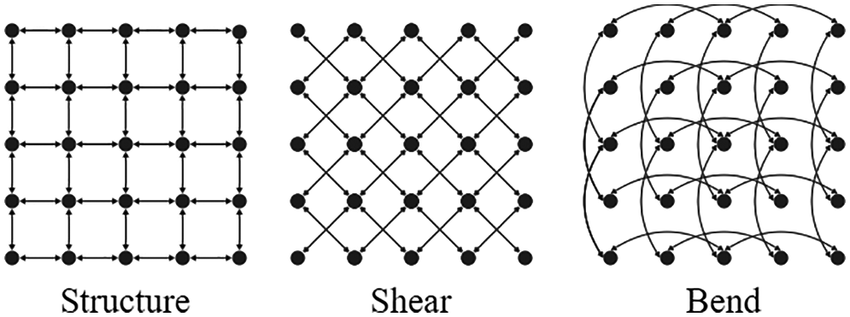
\includegraphics[scale=0.4]{springs.png}
	\caption{The types of springs typically used. Figure adapted from \protect\cite{springs}.}
	\label{fig:mss}
\end{figure}


 
\subsection{Position Based Dynamics}
With a valid simulation framework setup with mesh creation, particle vectors and the simulation loop working, the next thing to implement was position based dynamics. From this point, features were only created in the C++ version, as going back and forth between languages to implement the same things was not the best usage of time. As mentioned in Section \ref{lang}, the C++ program allows variables to be passed from C\# to the C++ app. This means a cloth simulation object can be created within C++ that assigns all the variables passed through, into properties of the cloth simulation object. Some of these variables can include vertex positions, triangle indices, solver iterations etc. There are two int variables that are used in switch statements within init and update, called scenario and algorithm. These variables switch into blocks of code to change how the simulation is run, scenario determines if the cloth is a hanging vertical cloth, or if its a horizontal cloth falling on a sphere. Algorithm changes which method is being used, between mass-spring, pbd and xpbd. \\

The PBD simulation loop is implemented in C++ based on the description of \cite{muller2007position}, as seen in Section \ref{lrPBD}.  Firstly, to handle particles the static particles that should be skipped, a simple check can be used on the $isStatic$ property of that particle in the loop, skipping that particle if the property is true. \\
The first step of the algorithm is updating the particles velocity by utilising delta time and the external forces of the system. In this case, gravity and wind. The idea of this ``for all vertices" block appears multiple times within the algorithm and can be translated to code as seen in Listing \ref{lst:cpploop}.

\begin{lstlisting}[caption={Updating particles velocity using external forces},label={lst:cpploop}]
for (int i = 0; i < _num_particles; i++)
{
	if (!_particles[i].is_static) {
		glm::vec3 external_forces = GRAVITY + (WIND_FORCE * wind_strength * std::sin(_total_time));
		_particles[i].velocity += _delta_time * _particles[i].inverse_mass * external_forces;
	}
}
\end{lstlisting}

Here, gravity and wind force are constants defined in the header file as \lstinline[language=C++]!const glm::vec3 GRAVITY = glm::vec3(0.0f,-9.81f,0.0f);! and \lstinline[language=C++]!const glm::vec3 WIND_FORCE = glm::vec3(0.0f, 0.0f, 1.0f);! respectively. This step is very similar to the first step of symplectic Euler in the mass spring system, calculating the new velocity. \\

Next, the velocity was damped to 99\% of its original value to simulate air friction. In the paper, the authors note that any form of damping can be used here. \\

The next step is to calculate the predicted position of the particle, based on the new velocity. This predicted position will then be iterated on for a specified number of times to get it closer to the goal position. This requires constraints which are key to the whole algorithm.
\subsubsection{Constraints}
\label{constraints} 
At its core, constraints in position based dynamics are similar to springs in a mass spring system, a way of adjusting particles so that they fit a certain constraint. Position based dynamics can be used for a vast range of deformable objects and can use constraints such as volume constraints. For cloth, structural and shear constraints are used.
\paragraph{Generating Constraints}\mbox{} \\ \\
Initially, constraints were held in a vector of uvec2, a glm type that holds two unsigned integers, and these integers would be the indices of the particles that are involved in this constraint. The constraints were generated using gridSize in a similar way to the mass spring system within a nested for loop, which can be seen in Listing \ref{lst:consGen}. 
\begin{lstlisting}[caption={The inner loop for constraint generation},label={lst:consGen}]
// Horizontal constraint
if (x < grid_size - 1)
{
	_structural_constraints.push_back(glm::uvec2(index, index + 1));
}

// Vertical constraint
if (y < grid_size - 1)
{
	_structural_constraints.push_back(glm::uvec2(index, index + grid_size));
}
\end{lstlisting}
This worked well for a basic PBD implementation but problems quickly arose when creating constraints on diagonals. In order to discuss the problems, it is necessary to explain constraint projection first. 
\paragraph{Constraint Projection}\mbox{} \\ \\
Once all constraints are generated and added to a vector, they can be used within the PBD simulation loop to iteratively move the particles to attempt to satisfy all constraints in the system. A integer variable called solver iterations was added and this controlled the amount of times to loop over the list of constraints and work on them again. This number typically ranged between 10 to 30 in testing, higher numbers resulted in more accurate simulations but also increased computational cost, as it had many more calculations to do each loop.\\

Constraint projection is simply the act of moving particles so that they satisfy the constraint. To satisfy a constraint in a cloth simulation like this, is achieved by having a goal distance. This goal distance was set to the distance between the two particles at the start of the simulation, the rest distance. This is where the first problem with the original design appeared. Originally, constraint projection had a hardcoded rest distance set to the spacing variable discussed back in Section \ref{creation}, this works fine for structural constraints, but when generating constraints in the diagonal, the rest distance of those two particles is equal to $\sqrt{r^2 + r^2}$, where r is the spacing variable. This was resolved by changing the data structure holding constraints to a vector holding a pair of uvec2 and float. This float would hold the rest distance of that constraint. \\

To actually project these constraints involves calculating two ${\Delta}p$, corrections that are applied to each particle to move it towards the goal, this can be seen in Figure \ref{fig:conproj}, these corrections would be weighted on the inverse masses of each particle. This is especially useful for static particles, as the inverse mass of those are set to 0. The formula for calculating these corrections turns out to be a special case of the general constraint method in the paper, and becomes: 
\[{\Delta}p_1=-\frac{w_1}{w_1+w_2}(\lvert p_1-p_2 \rvert -d)\frac{p_1-p_2}{\lvert p_1-p_2 \rvert}\] 
\[{\Delta}p_2=+\frac{w_2}{w_1+w_2}(\lvert p_1-p_2 \rvert -d)\frac{p_1-p_2}{\lvert p_1-p_2 \rvert}\] 
Where $w$ is the inverse mass, $p$ is the predicted position and $d$ is the rest distance.
Once these corrections are calculated, they are added to the predicted position of the respective particle during the loop. \\

Another aspect of constraints is stiffness. In the PBD implementation, stiffness is obtained by multiplying ${\Delta}p$ by $k\in[0...1]$. This works, but the effect of this stiffness is non-linear with multiple solver iterations. This can be fixed by calculating $k'=1-(1-k)^{1/n_s}$, where $n_s$ is the number of solver iterations. This is then used to multiply ${\Delta}p$.
\begin{figure}
	\centering
	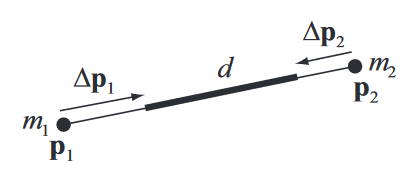
\includegraphics[scale=0.5]{constraint.png}
	\caption{Projection of a constraint between two particles. Figure adapted from \protect\cite{muller2007position}.}
	\label{fig:conproj}
\end{figure}
\paragraph{Improved Constraint Generation}\mbox{} \\ \\	
A problem with the earlier constraint generation was that it relied on the grid size variable. This means it would only work for a X by X square mesh, this is obviously not ideal, so the constraint generation needed to be reworked. One way to do this is by using the triangle data. Relying on the fact that the triangle data passed in is sorted by adjacency, we can use the indices of these to generate the constraints. \\

This is achieved by looping through the number of triangles, incrementing by two each time, and working on two triangles at once. The first triangle's indices can be retrieved with the index, while the second triangle's indices can be retrieved with index + 1. With all 6 vertices of these two triangles, it is easy to create both structural and shear constraints in this manner. \\

Sets of pairs of ints were created to hold temporary constraints. There were two main reasons for this approach. In C++, elements of a set have to be unique, this is to avoid creating duplicate constraints, e.g. $C(p_1,p_2)$ and $C(p_2,p_1)$. Using a function called minmax, the pair of ints can be sorted so that the lowest value is first. This is used in tandem with the property of sets to make sure each constraint is only created once. A full example is: a constraint between particle index 1 and index 20 is created as $(1,20)$ and inserted into the set. When the loop goes to create a constraint between index 20 and index 1, minmax will turn it into $(1,20)$ and it won't be added to the set as it already exists in there. \\

Once the temporary sets are created, they can be looped through and inserted into the constraints vector along with the rest length between the two particles. With this new constraint generation, any mesh can be used so long as the triangle data is sorted by adjacent triangles.
\subsubsection{Updating Position and Velocity}
Once the constraints have been projected for a given number of times, it is necessary to set the particles new velocity and position. The velocity can be calculated as: $v_1=\frac{p_1-x_1}{dt}$, where $p_1$ is the predicted position, $x_1$ is the current position and $dt$ is delta time. After this, the particles position is simply updated to match the calculated predicted position. It is also necessary to update the positions vector that is passed back to Unity, as this will update the meshes vertex positions. \\

With this entire loop, the PBD implementation correctly works to simulate cloth with great performance and good accuracy. 
	
\subsection{Extended Position Based Dynamics}
Now that PBD is successfully implemented, the XPBD extension can also be implemented. This was added as another algorithm type, so that it is easy to switch between them. The first major improvement that XPBD offers is the usage of substeps.
\subsubsection{Substeps vs Solver Iterations}
In the XPBD paper, the authors found that spending the fixed time budget of one frame is much more effective by using substeps instead of solver iterations. In essence, XPBD encapsulates the whole PBD simulation in a loop of substeps, instead of wrapping the constraint projection inside solver iterations. This means that constraints are processed only once per substep. However, multiple substeps are executed within a single simulation loop, allowing for iterative processing of constraints across the entire simulation. \\

After understanding XPBD's approach to simulating, it is clear that the way delta time is handled needs to be tweaked. Instead of using delta time within the loop, a new measurement of delta time substeps is calculated as ${\Delta}t_s=\frac{{\Delta}t}{n}$, where $n$ is the number of substeps. This new variable represents the duration of each substep. \\

This new approach of using substeps solves the original problem with PBD, the constraint stiffness depending on time step. 
\subsubsection{Stiffness through a Compliance Factor}
With XPBD, there is also an extension to how constraint stiffness is altered. PBD handles stiffness by multiplying the correction by a stiffness variable between 0 and 1 as discussed in Section \ref{constraints}. With XPBD, a compliance factor is used. Within XPBD, compliance represents the inverse of physical stiffness, meaning the constraint is infinitely stiff when compliance ($\alpha$) is 0. Compliance fits into the correction equation as so:
\[{\Delta}p_1=-\frac{w_1}{w_1+w_2+\frac{\alpha}{{\Delta}t^2}}(\lvert p_1-p_2 \rvert -d)\frac{p_1-p_2}{\lvert p_1-p_2 \rvert}\] 
With this extra factor, this way of applying stiffness to a constraint is much preferred over the original PBD, as it doesn't depend on time steps any more.
\subsection{User Cloth interaction}
An additional feature created was user interaction through the mouse. This feature would allow the user to click, hold and drag a particle around in space. When the mouse button is held, the chosen particle acts as a static particle with infinite mass, allowing the constraints to function as if this particle was pinned. \\

The way this is achieved is through Unity's raycasting support. If the mouse is clicked, a ray is cast from the camera in the direction of the mouse cursor. If this ray hits the collider of the cloth mesh, the exact position of this collision is calculated. Another helper function was created to find the nearest particle to this position. This is a minimisation function that loops through all particles to calculate which particle is closest to the collision point, the particle's index is then returned. Finally, this mouse position is converted from screen space to world space, with the z coordinate being the distance from camera to the cloth. The particle's index and mouse position are then passed to C++ where it is utilised in the simulation loop. \\

The code for user interaction is implemented within the regular Update method. This is because user interactions such as mouse clicks can happen every frame, and thus need the additional responsiveness from Update compared to FixedUpdate. If this was implemented in FixedUpdate, there could be situations where a mouse click occurs between two consecutive FixedUpdate calls, resulting in a missed input. \\

One additional integer is also passed through, stopGrabbingIndex. This is needed to revert the particle's properties back to normal when the mouse click is released. Two if statements that facilitate the grabbing feature can be seen in Listing \ref{lst:user}.
\begin{lstlisting}[caption={Modifying particles from user interaction},label={lst:user}]
if (stop_grabbing_index != -1)
{
	_particles[stop_grabbing_index].inverse_mass = 1.0f;
	_particles[stop_grabbing_index].is_static = false;
}
if (selected_particle_index != -1)
{
	_particles[selected_particle_index].inverse_mass = 0.0f;
	_particles[selected_particle_index].is_static = true;
}	
\end{lstlisting}
It is necessary to set the mass as well as the static property, to allow the constraints between this held particle and other particles to function properly, as the constraints are weighted based on both particles mass. Inside the PBD/XPBD loop, when calculating the predicted position, if the current particle is held, then the predicted position is just set to the mouse world position, instead of calculating it based on velocity. With this feature implemented, the user is able to click and drag any particle in the mesh, allowing the cloth to be tested for situations like folding and stretching. This can be seen in Figure \ref{fig:drag}.
\begin{figure}
	\centering
	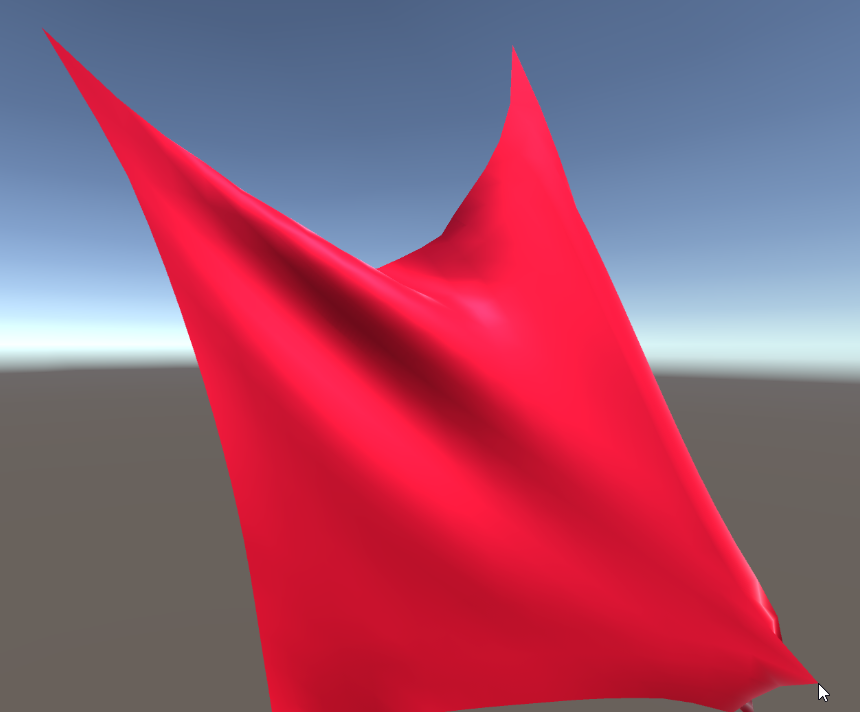
\includegraphics[scale=0.5]{drag.png}
	\caption{Hanging cloth mesh being dragged by a corner particle}
	\label{fig:drag}
\end{figure}
\subsection{Cloth and Sphere Collision}
\label{collision}
Collision was the next feature to be implemented for use in the scenario of a horizontal cloth falling on top of a static sphere. First, a simple sphere object was created within Unity using the sphere primitive. This will have two relevant properties: Sphere centre and sphere radius. There are many ways to do collision in physics simulations and the implementation depends on the scenario and usage of it. It is mentioned by the authors in the original PBD paper that position based approaches have an advantage compared to normal methods because of how easy it is to implement collision and response. They do this by creating collision constraints. With collision between cloth and a small rigid body, two way collision is required, due to the fact that the small object could potentially fall through the cloth. In this situation, only collision between the cloth and the sphere is needed, due to the sphere being large. \\

The way this collision and response is handled is by checking each particle's predicted position during the PBD/XPBD loop. A vector between the position of the sphere's centre and the predicted position can be calculated. If the length of this vector is smaller than the radius of the sphere then the particle has collied with the sphere. The depth of this collision is then calculated and multiplied with the normalised vector calculated earlier. This delta can then be added to the predicted position, to move the particle outside the sphere in the direction of this vector. This can be coded very easily as seen in Listing \ref{lst:col}. 
\begin{lstlisting}[caption={Sphere collision function},label={lst:col}]
void ClothSim::CollisionWithSphere()
{
	for (int i = 0; i < _num_particles; i++)
	{
		// Calc the vector from particle to sphere centre, if its shorter than sphere radius then a collision has occured
		glm::vec3 particle_to_centre = _particles[i].predicted_position - _sphere_centre;
		float length = glm::length(particle_to_centre);
		
		if (length < _sphere_radius)
		{
			float depth = _sphere_radius - length;
			depth += 0.0001f;
			glm::vec3 delta = glm::normalize(particle_to_centre) * depth;
			_particles[i].predicted_position += delta;
		}
	}
}

\end{lstlisting}
The $0.0001f$ that is added to the depth is known as depth bias. It is used to make sure the particles aren't just moved directly onto the sphere. This helps to avoid the cloth getting stuck, as it might still be colliding on the very next frame. It also helps with z-fighting issues, this will be discussed in Section \ref{spherescene}.
\section{Results and Discussion}
Now that the entire implementation is finished, it is necessary to test and experiment with variables to fully gauge the simulations effectiveness. This will mean comparing the C++ and C\# implementations, discussing the two scenarios, discussing the recorder feature that was implemented and analysing the visuals of the simulation.
\subsection{C++ vs C\#}
\label{cppcomp}
As discussed in Section \ref{mss-metho}, the mass spring system was implemented in both C++ and C\#. This will allow for testing of both versions with the same setup, to check performance. Inside Unity's Update function, a quick if/else was created to sum up and average the frames over the first 10 seconds of simulation. This will be used over 5 runs of both C++ and C\# to check the true average frame time for both implementations. Frame time is a common metric in real time graphics and it represents the time taken to render a frame.  Before testing, it is expected that the C++ version will outperform C\#, due to the efficiency of C++ and not having to deal with garbage collection in C\#. This experiment will be conducted on 20x20 mesh of spacing 0.5, a 100x100 mesh of spacing 0.125 and finally, a 150x150 mesh of spacing 0.125. The results of the first experiment can be seen in Table \ref{tab:lang}. \\
\begin{table}[htbp]
	\centering
	\begin{tabular}{|c|c|c|} % Specifies three columns with centered content, and vertical lines between columns
		\hline % Horizontal line at the top of the table
		Run \# & C\# frame time (ms) & C++ frame time (ms)\\ % Table header row
		\hline % Horizontal line below the header row
		1 & 1.695 & 1.569 \\ 
		2 & 1.723 & 1.557 \\ 
		3 & 1.732 & 1.521 \\ 
		4 & 1.711 & 1.567  \\ 
		5 & 1.670 & 1.528  \\ 
		\hline
		Average & 1.706 & 1.548 \\ 
		\hline % Horizontal line at the bottom of the table
	\end{tabular}
	\caption{Frame time comparison between C\# and C++ for a mass spring system of 20x20 particles} % Table caption
	\label{tab:lang}
\end{table}

It can be seen here that on average, the C++ frame time is 0.158ms faster, which is a sizeable improvement. To analyse with a bigger mesh, a 100x100 is also tested with a spacing of 0.125. This second mesh will have 10,000 vertices and 19,602 triangles, compared to 400 vertices and 722 triangles of the first experiment. The result of this second experiment can be seen in Table \ref{tab:lang2}. \\
\begin{table}[htbp]
	\centering
	\begin{tabular}{|c|c|c|} % Specifies three columns with centered content, and vertical lines between columns
		\hline % Horizontal line at the top of the table
		Run \# & C\# FPS & C++ FPS \\ % Table header row
		\hline % Horizontal line below the header row
		1 & 435.59 & 494.08 \\ 
		2 & 437.19 & 499.90 \\ 
		3 & 441.57 & 499.25 \\ 
		4 & 427.20 & 498.88  \\ 
		5 & 425.99 & 499.53  \\ 
		\hline
		Average & 433.51 & 498.13 \\ 
		\hline % Horizontal line at the bottom of the table
	\end{tabular}
	\caption{FPS comparison between C\# and C++ for a mass spring system of 100x100 particles} % Table caption
	\label{tab:lang2}
\end{table}

With this second experiment, the fps on both versions are lower as expected, and the C++ version still outperforms the C\#, this time by 65 fps on average. It has to be noted that at higher particle size, this mass spring system implementation is extremely elastic and doesn't truly represent any real world cloth material, and with the problem of instability at higher spring constants, it is unable to simulate accurate cloth. This could potentially be due to only structural springs being implemented, and there not being enough forces to keep the particle mesh in its original shape. \\

A final test using a mesh of 150x150 particles and a spacing of 0.125 was performed to test the extremes of both implementations. The results of testing both implementations with this mesh can be seen in Table \ref{tab:lang3}.\\
\begin{table}[htbp]
	\centering
	\begin{tabular}{|c|c|c|} % Specifies three columns with centered content, and vertical lines between columns
		\hline % Horizontal line at the top of the table
		Run \# & C\# FPS & C++ FPS \\ % Table header row
		\hline % Horizontal line below the header row
		1 & 69.96 & 187.19 \\ 
		2 & 70.29 & 188.69 \\ 
		3 & 74.30 & 187.78 \\ 
		4 & 76.29 & 192.00  \\ 
		5 & 73.39 & 190.79  \\ 
		\hline
		Average & 72.85 & 189.29 \\ 
		\hline % Horizontal line at the bottom of the table
	\end{tabular}
	\caption{FPS comparison between C\# and C++ for a mass spring system of 150x150 particles} % Table caption
	\label{tab:lang3}
\end{table}

With this final experiment, there was a noticeable drop off in fps compared to the previous two experiments, yet C++ remained well ahead vs C\#. On average, C++ outperformed by 116 fps, leading to the conclusion that fps saved was proportional to the mesh size. This makes sense, as when the amount of calculations and vector manipulation increases, C++ will be saving more time compared to C\#. For the mass spring system, any higher resolution meshes and the fps begins to suffer heavily as a result of the increased computations required.\\

As C++ is clearly superior than C\# at physics simulations, it was clear that the rest of the project was to be implemented only in C++ and to not waste development time repeating it in C\#. The rest of the results will be solely resulting from the C++ code, except from features like recording videos from within Unity.
\subsection{Recording Feature}
To properly evaluate the simulations, it is necessary to record different algorithms and scenarios to be able to compare them. Unity recorder is a plugin within Unity that allows for video's and screenshots to be taken of projects. Usually it is manually used through a plugin window but it also provides an API to allow for scripts to manage recording. \\

With this, a mass-recording system was successfully implemented within the C\# script. It uses a new class called recordParameters that sets variables to be tested, such as the number of PBD solver iterations, its stiffness and scenario etc. A generate filename function was also implemented that takes in a recordParameters object and generates a unique filename from its properties. The way this recording feature was designed allowed for lots of different experiments to be queued up and recorded in succession. In Unity's update, it checks if it is currently recording, if it isn't it takes the next pending experiment and starts it. The recording folder within the project can now hold all the experiments that are clearly identified with the filename as seen in Figure \ref{fig:recs}.

\begin{figure}
	\centering
	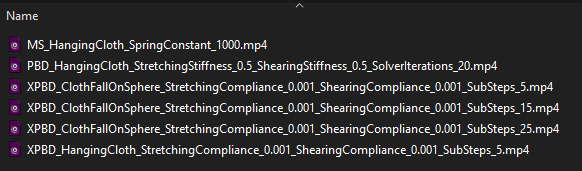
\includegraphics[scale=0.8]{recs.png}
	\caption{The folder of experiment recordings.}
	\label{fig:recs}
\end{figure}


\subsection{Scenarios}
In this project, two distinct scenarios were implemented to test aspects of cloth simulation that are common use cases for it, such as a hanging cloth acting as things such as curtains or flags. The second scenario being a horizontal cloth falling onto a rigid sphere. This was to test how the constraints function when including collision. 
\subsubsection{Hanging Cloth}
The first scenario is the basic hanging cloth scenario. This mesh was created vertically, so 0.0f was value for the z-axis in every coordinate when initialising. There were two main ways the cloth was pinned in testing. The first being the top two corner particles being static, this would emulate a cloth such as clothes being pinned with two pegs, or a cape. The second way was the entire top row of particles being pinned, emulating a flag. Overall, the first method was used much more in testing as it allows the constraints to be shown better, and displays interesting properties regarding the top row of particles. \\

Wind was also used in this scenario to apply an additional force than just gravity. Allowing the display of a system with multiple forces interacting with multiple particles. This wind was a simple vector with magnitude 1.0 in the z direction, blowing the cloth away and towards the camera. The magnitude changed between 1.0 and -1.0 using a sine function with total simulation time as the factor. \\

A useful property of Unity is the range property of public variables. If a range is applied above a public variable as so:
\begin{lstlisting}[caption={Unity's range feature},label={lst:rng}]
[Range(0f, 100f)]
public float windStrength = 1.0f;
\end{lstlisting}
It will allow the user to manipulate this variable in real time with a slider. This feature is crucial in analysing different setups to display how properties such as stiffness or wind affect the simulation.

\paragraph{Mass-Spring System} \mbox{} \\
In the mass spring system version of the hanging cloth, a variable to test the impact of is spring constant. As explain in Section \ref{mss-metho}, the spring constant multiplies the force applied by the springs. A higher spring constant results in a stiffer system, while a lower results in a loose one. In Figure \ref{fig:msscomp}, three versions of the simulation can be seen with spring constants of 500, 1000 and 1500 from left to right. The lower spring constant cloth sagging under the force of gravity while the higher spring constants hold up more. Changing this variable can help the developer tune the cloth to have different properties depending on the use case.

\begin{figure}
	\centering
	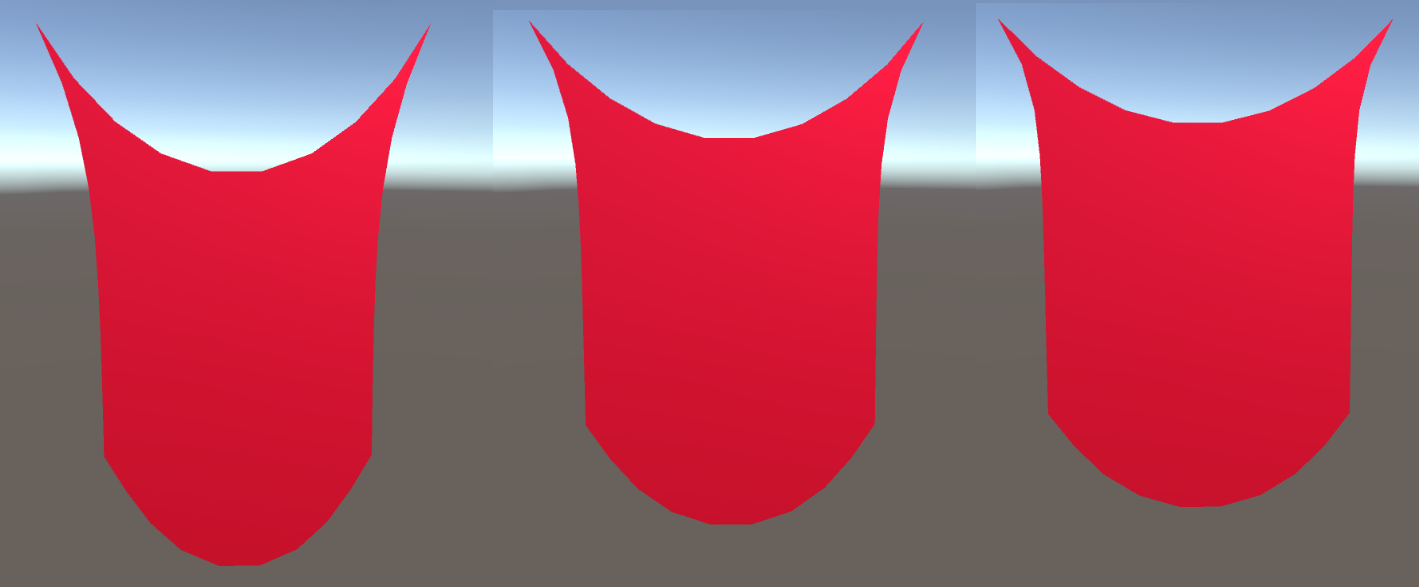
\includegraphics[scale=0.35]{msscomp.png}
	\caption{Three versions of the mass spring system, with spring constants of 500,1000 and 1500 left to right}
	\label{fig:msscomp}
\end{figure}

\paragraph{Position Based Dynamics} \mbox{} \\
The position based dynamics implementation within this project has a few more parameters that can be tuned and experimented with. These can include: delta time, structural stiffness, shearing stiffness and solver iterations. In the original paper, one problem was that constraint stiffness was heavily impacted by the time step and solver iterations. More specifically, the system would get more stiff as the solver iterations increased, or time step decreased. Within Unity, the fixed time step is easily modifiable in the project settings, and was normally set at 0.02s or 50 fixed updates per second. This can be then tested to verify. The only variable changing is fixed time step, the others are: 
\begin{itemize}
	\item Solver iterations = 20
	\item Stretching stiffness = 0.5
	\item Shearing stiffness = 0.5
\end{itemize}

The three time steps tested were 0.04, 0.02 and 0.01, or 25, 50 and 100 updates per second respectively. In Figure \ref{fig:pbdts} it is quite apparent the severe impact that fixed time step has on the original PBD implementation. This is problematic as it requires the developer to retune all stiffness properties for different time steps, requiring much more work. This was one of the improvements that XPBD had over the original, stiffness independent of time step. \\

For the problem of iteration count, PBD attempts to mitigate this with the stiffness term that involves iteration count as explained in Section \ref{constraints} but in the XPBD paper, the authors note that this doesn't converge to a well defined solution in the presence of multiple constraints. For this project, it successfully decouples stiffness from iteration count but for a more advanced simulation it would pose issues. \\
\begin{figure}
	\centering
	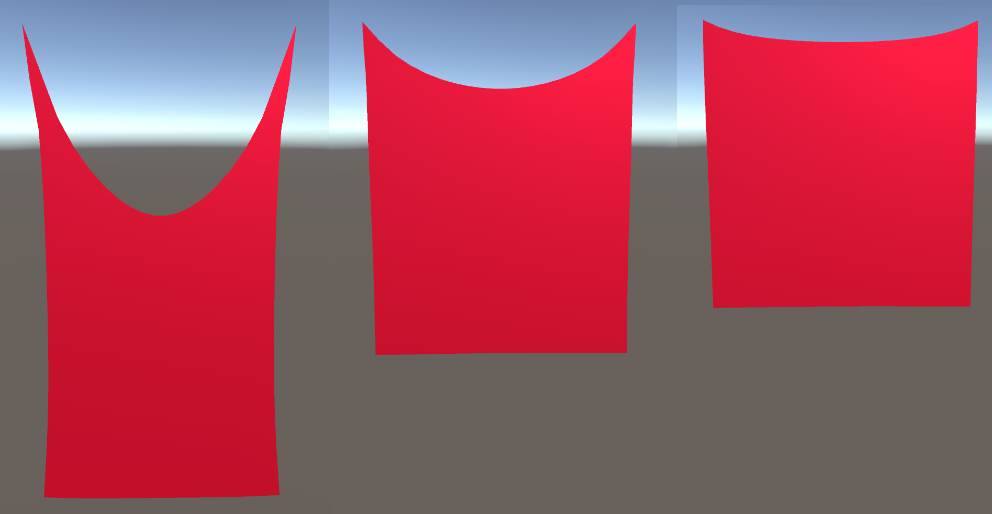
\includegraphics[scale=0.5]{pbdtscomp.png}
	\caption{Testing the time step stiffness issue with original PBD, with time steps of 0.04, 0.02 and 0.01 left to right}
	\label{fig:pbdts}
\end{figure}

Having both structural and shear stiffness being variable allows for lots of variation in the end cloth, for example in Figure \ref{fig:pbdcomp}, the cloth on the left has a structural stiffness of 1, and a shear stiffness of 0, while the cloth on the right has both structural and shear stiffness of 1. The cloth with both stiffness set to 1 acts extremely stiff and would be suitable to represent objects such as paper or card, while the other acts more naturally like clothes or flags.
\begin{figure}
	\centering
	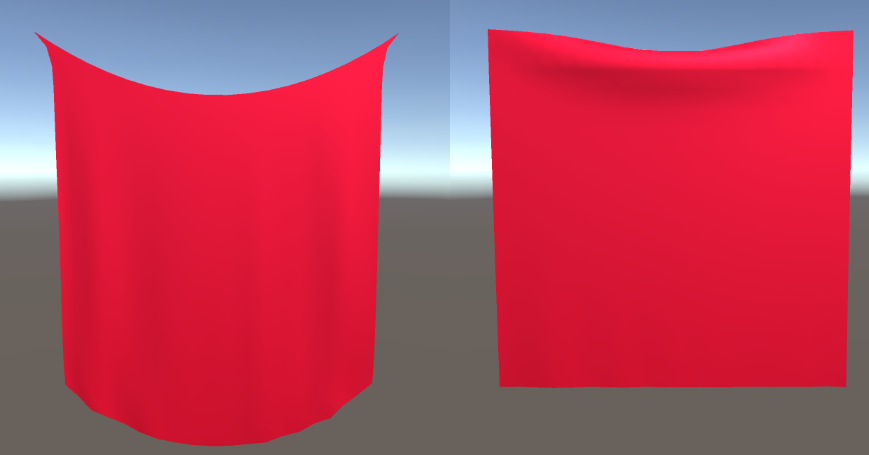
\includegraphics[scale=0.5]{pbdcomp.png}
	\caption{Cloth with different stiffness values}
	\label{fig:pbdcomp}
\end{figure}
\paragraph{Extended Position Based Dynamics} \mbox{} \\
Now, it is vital to test the hanging cloth using the extended position based dynamics method. On the whole, the overall simulation loop is extremely similar with a few improvements, substeps and stiffness compliance. Substeps were the first to be tested, the other parameters were as follows:  
\begin{itemize}
	\item Stretching compliance = 0.0005
	\item Shearing compliance = 0.0005
	\item Wind strength = 0.7
\end{itemize}
The substeps would be tested at 1, 20 and 40. This means that for every fixed update, the simulation loop would repeat for the number of substeps. It can be expected that as substeps increase, overall simulation accuracy will increase. This will come with a computational cost so the expected fps will also be lower as substeps increase. Wind is utilised in this experiment to have an additional force on the cloth to inspect how substeps affect the constraint projection. \\

The recorder feature was utilised here to run these three tests, as it was easy to change substeps in the recorder class. In Listing \ref{lst:exp}, is an example of how multiple experiments were run, keeping most of the properties the same but changing substeps. \\ \\ \\
\begin{lstlisting}[caption={Utilising the recorder feature},label={lst:exp}]
for (int i = 0; i < 3; i++)
{
	int[] subs = new int[]{1,20,40};
	var rp = new RecordParameters
	{
		algorithm = 2, // XPBD
		scenario = 0, // HangingCloth
		xpbdStretchingCompliance = 0.0005f, 
		xpbdShearingCompliance = 0.0005f, 
	};
	rp.xpbdSubsteps = subs[i];
	rp.filename = $"{GenerateFilename(rp)}";
	
	// Add the recording settings to the pendingExperiments list
	pendingExperiments.Add(rp);
}
\end{lstlisting}
When analysing these three, there are two main aspects to look at, visuals and FPS. In Table \ref{tab:sub}, the FPS of each test is averaged over 10 seconds. It can be seen that increasing the number of substeps has a drastic effect on performance, with the 40 substeps experiment dipping to 20 FPS.\\
\begin{table}[htbp]
	\centering
	\caption{Substeps and FPS Data}
	\label{tab:sub}
	\begin{tabular}{cc}
		\toprule
		Substeps & FPS \\
		\midrule
		1 & 599.04 \\
		20 & 306.58 \\
		40 & 20.67 \\
		\bottomrule
	\end{tabular}
\end{table}

The visuals of the simulation are also affected. The 1 substep experiment overall looks too smooth and when moved with the mouse interaction, it has a delay before it moves. This makes sense, as the constraints are only projected once in each fixed update, so the time taken to satisfy all constraints will be considerably longer. This also means the cloth takes longer to come to rest. \\

This is fixed in the 20 substep version, as the constraints can be projected multiple times in one fixed update, leading to the cloth overall looking more physically realistic. It also fixes the issue of the delay before moving and it comes to rest quicker. \\

The 40 substeps version has taken quite the performance hit, leading to overall less appealing visuals through the lower fps, so the ideal substeps for this project is around 20. \\

Next, the time step issue from the original PBD can be tested to see if the XPBD version has fixed it. The same time step experiments used in the PBD paragraph will be used here, 0.04,0.02 and 0.01. Before experimenting, it is expected that changing the time step will have no effect on the stiffness of the simulation, due to the new compliance factor in XPBD. The results of these experiments can be seen in Figure \ref{fig:xpbdcomp}.
\begin{figure}
	\centering
	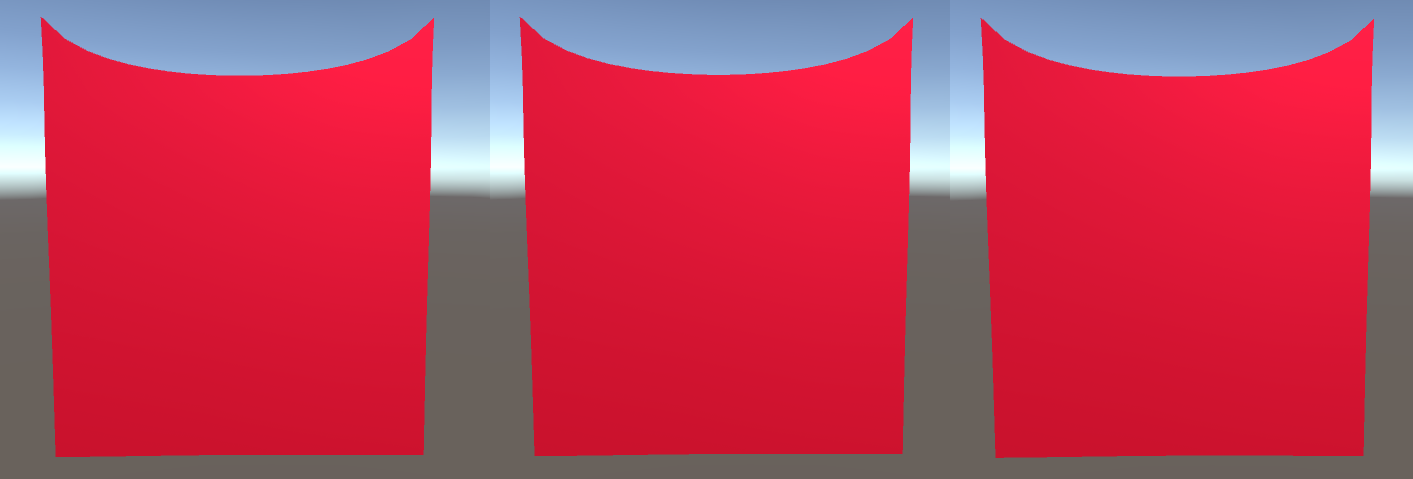
\includegraphics[scale=0.35]{xpbdtscomp.png}
	\caption{Time step stiffness problem resolved in XPBD}
	\label{fig:xpbdcomp}
\end{figure}
With XPBD, the stiffness of the system now doesn't depend on the time step of the project which is a very useful improvement. Now, the developers can tune the XPBD simulation's stiffness parameters to suit a wide range of time steps without having to change the parameters for different time steps.
\subsubsection{Cloth falling on Sphere}
\label{spherescene}
The second scenario in this project is a horizontal cloth falling onto a static, rigid sphere. This scenario is made to test how the constraints function in a simulation where collision is also a factor. The horizontal cloth was generated in a similar way to the vertical cloth. When creating the vertex coordinates, the y coordinate was set to 0 instead of the z like so: \\ \lstinline{vertices[i] = new Vector3(x * spacing, 0, y * spacing);}\\

The sphere is created in Unity, with a radius of 2.5f. The sphere centre can be obtained in C\# by acquiring the transform position of the sphere game object, these two variables are then passed to C++ to be used in the collision code discussed in Section \ref{collision}. \\

Initially, there was an issue where the sphere object could be seen through the cloth when they were colliding. This is a known issue in computer graphics called stitching or z-fighting. It occurs when two objects within a scene have very similar distances to the camera, which causes issues when deciding what object to render first. This problem can be visualised in Figure \ref{fig:zfight}. \\
\begin{figure}
	\centering
	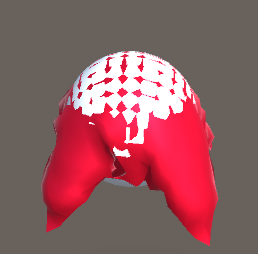
\includegraphics[scale=0.5]{zfight.png}
	\caption{Z-fighting issue when rendering two colliding objects}
	\label{fig:zfight}
\end{figure}

To address this issue, a novel approach was implemented in this project. In the cloth shader, an additional rendering pass was used alongside the command ``ZTest Always". This command specifies the depth test function for determining if a pixel should be drawn on not. By assigning ``Always" to it ensured that the cloth will always be rendered on top of other objects, regardless of position. \\

However, this alone wouldn't be enough to solve the issue, as the cloth would continue to be rendered on top of the sphere, even when it falls behind it. To overcome this challenge, the shader used for the sphere was modified to a transparent one. This alteration effectively transformed the appearance of the sphere into glass-like, allowing the cloth to be rendered behind it without appearing out of place. The result of this approach can be seen in Figure \ref{fig:spherefixed}. \\
\begin{figure}[h]
	\centering
	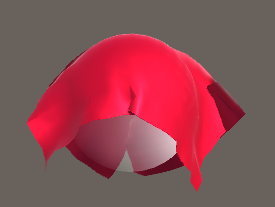
\includegraphics[scale=0.5]{spherefixed.png}
	\caption{The glass sphere approach to solve z-fighting}
	\label{fig:spherefixed}
\end{figure}
With this implementation, the sphere successfully collides with the sphere and reacts in a physically plausible way, sliding off the sphere. With friction, the cloth would most likely stay on top of the sphere, but it was not implemented in this project. The way the sphere interacts with the cloth using such simple collision code, showcases the effectiveness of XPBD's constraints in simulating realistic cloth dynamics.
\subsection{Discussion}
With these experiments conducted, the overall effectiveness of PBD and XPBD can be discussed. 

\section{Reflection}
4.1 Is there clear reflection on the project process, showing achievements in overcoming difficulties?\\
4.2 Are the outcomes and deliverables evaluated with respect to the project aims and to the work of others?\\
4.3 Is it clear what the student would do differently with hindsight?\\
4.4 Is it clear what future work could be done to the project? \\

Although PBD and XPBD were explored to a high degree in this project, there is much room for improvements and additional features to be implemented. 

\section{Conclusion}
f
\bibliographystyle{apacite}
\bibliography{bibliography}

%you can crate this on a extra tex document just like the title or any other part of the document.
\newpage
\begin{appendices}
\begin{minipage}{\textwidth}
	
\includepdf[offset=0 -2cm,scale=0.65,pages=1,pagecommand={\section{Project Overview}}]{appendices/IPO.pdf}
\end{minipage}

\includepdf[scale=0.65,pages=2,pagecommand={}]{appendices/IPO.pdf}
\begin{subappendices}

\subsection{Example sub appendices}
...
\end{subappendices}

\section{Second Formal Review Output}
Insert a copy of the project review form you were given at the end of the review by the second marker

\section{Diary Sheets (or other project management evidence)}
Insert diary sheets here together with any project management plan you have

\section{Appendix 4 and following}
insert content here and for each of the other appendices, the title may be just on a page by itself, the pages of the appendices are not numbered, unless an included document such as a user manual or design document is itself pager numbered.
\end{appendices}

\end{document}
